% Appendix --- category-count (cardinality) tuning and reproducibility.
% The cardinality curve transforms the base macro F1 into an adjustable
% operating point; the figure is the real winner_cardinality_curve.png.
\appendix
\section{Category-Count Tuning: Quality vs.\ Coverage}
\label{app:cardinality}

A practically relevant deployment decision is how many crop categories
to commit to. The final ensemble classifies all 18 PASTIS-R classes,
but six minority crops with ambiguous phenology pull down the global
macro F1. The cardinality curve answers a concrete business question:
if the system commits to only the $K$ best-resolved crops, what average
quality is achieved and what fraction of real parcels is covered?

The methodology is honest: the ranking of which class to drop is
determined on out-of-fold probabilities from the training set, and the
metric is measured on the held-out fold restricted to the retained
classes, so the improvement is not a post-hoc selection artefact.
Figure~\ref{fig:cardinality} shows the full curve.

\begin{figure}[htbp]
    \centering
    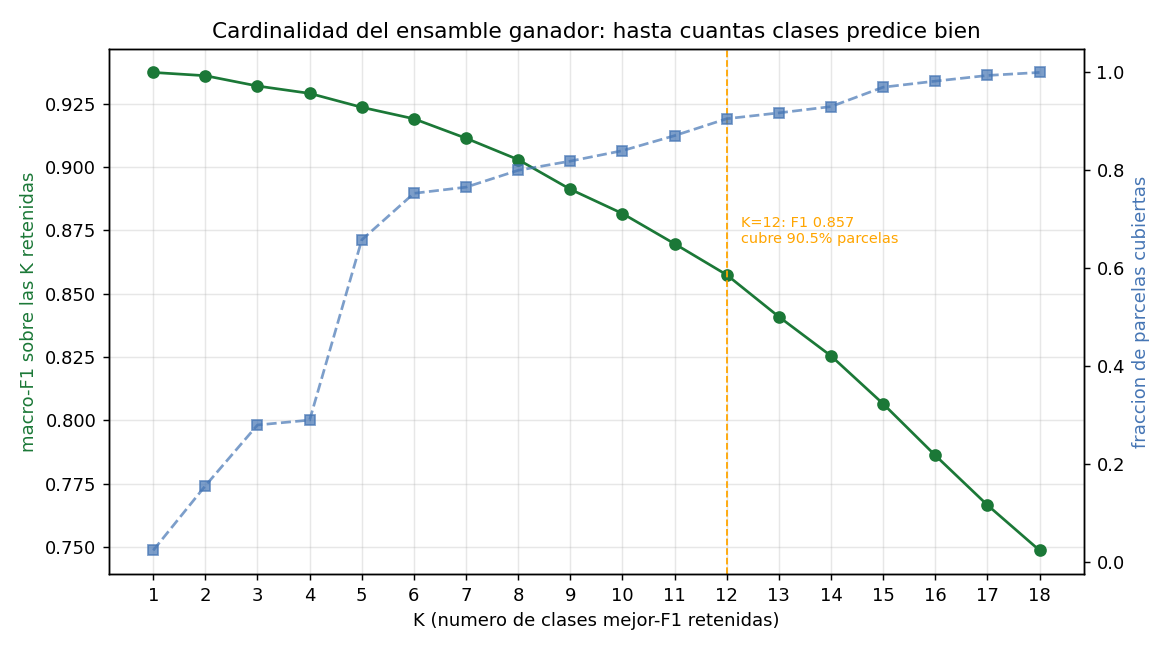
\includegraphics[width=0.9\columnwidth]
      {../reports/ensemble/figures/us043_farslip/winner_cardinality_curve.png}
    \caption{Cardinality curve of the final model (Stacking~+~FarSLIP).
    The elbow around $K=8$--$9$ marks the optimal quality/coverage
    trade-off for most use cases.}
    \label{fig:cardinality}
\end{figure}
% src(figure): reports/ensemble/figures/us043_farslip/winner_cardinality_curve.png
% src(curve data): reports/ensemble/metrics/us043_winner_cardinality_curve.csv

The curve yields concrete operating points (per-$K$ macro F1 and
cumulative support share read from the held-out cardinality analysis).
At full cardinality ($K=18$) the model attains macro F1 0.7486 over
100\% of parcels. Trimming to the 12 best-resolved crops raises macro
F1 to 0.8574 while still covering 90.5\% of real parcels; the
\texttt{france-9} operating point ($K=9$) reaches macro F1 0.8912 at
81.9\% coverage; and a focused high-precision mode at $K=8$ exceeds
macro F1 0.9029 over 80.0\% of parcels. The elbow sits around
$K=8$--$9$, the optimal quality/coverage trade-off for most use cases.
No retraining is required: the stacking meta-model already produces
per-class probabilities, so the category threshold is applied
dynamically in production.

\section{Spatial Neighbourhood Blending: A Null Result}
\label{app:neighbourhood}
We also tested whether convexly blending each parcel's champion
posterior with the mean posterior of its $k$ spatial neighbours
(centroid $k$-NN in EPSG:2154, neighbour posteriors only, no
ground-truth leak) improves the held-out macro F1. It does not: on the
\texttt{france-9} label space the change is $+0.0002$ macro F1 at best,
within noise, and the 18-class space moves by at most a few thousandths
before degrading as the blend weight grows. We report this as an
honest null result: the spatial context that neighbourhood blending
would add is already absorbed by the AlphaEarth annual
embedding~\cite{brown2025alphaearth}, which encodes regional context at
the parcel level, so an explicit neighbourhood term is redundant.
% src: reports/ensemble/metrics/ec_neighborhood_result.json
% (champion france9 0.9121; alpha sweep delta_f1_macro_france9 ~ +/-0.002, noise)

\section{Reproducibility Artefacts}
\label{app:repro}

Every quantitative result is anchored to a versioned artefact:

\begin{itemize}[leftmargin=*]
    \item Individual segmentation (fold-5):
    \texttt{reports/segmentation/metrics/model\_comparison\_fold5.csv}.
    \item Ensembles:
    \texttt{reports/ensemble/us043\_farslip\_summary.json} and
    \texttt{reports/ensemble/metrics/comparison\_us040.csv}.
    \item FarSLIP feature space:
    \texttt{reports/farslip/metrics/us037\_farslip\_fiel\_vs\_alphaearth.csv}.
    \item France$\rightarrow$Catalonia transfer:
    \texttt{reports/segmentation/sen4agrinet\_transfer\_result.json}.
    \item Datasets (DVC): \texttt{data/sen4agrinet.dvc},
    \texttt{data/transfer/eurocropsml.dvc}.
\end{itemize}
